\section{What Does Not Work}

\begin{figure}[t]
\centering
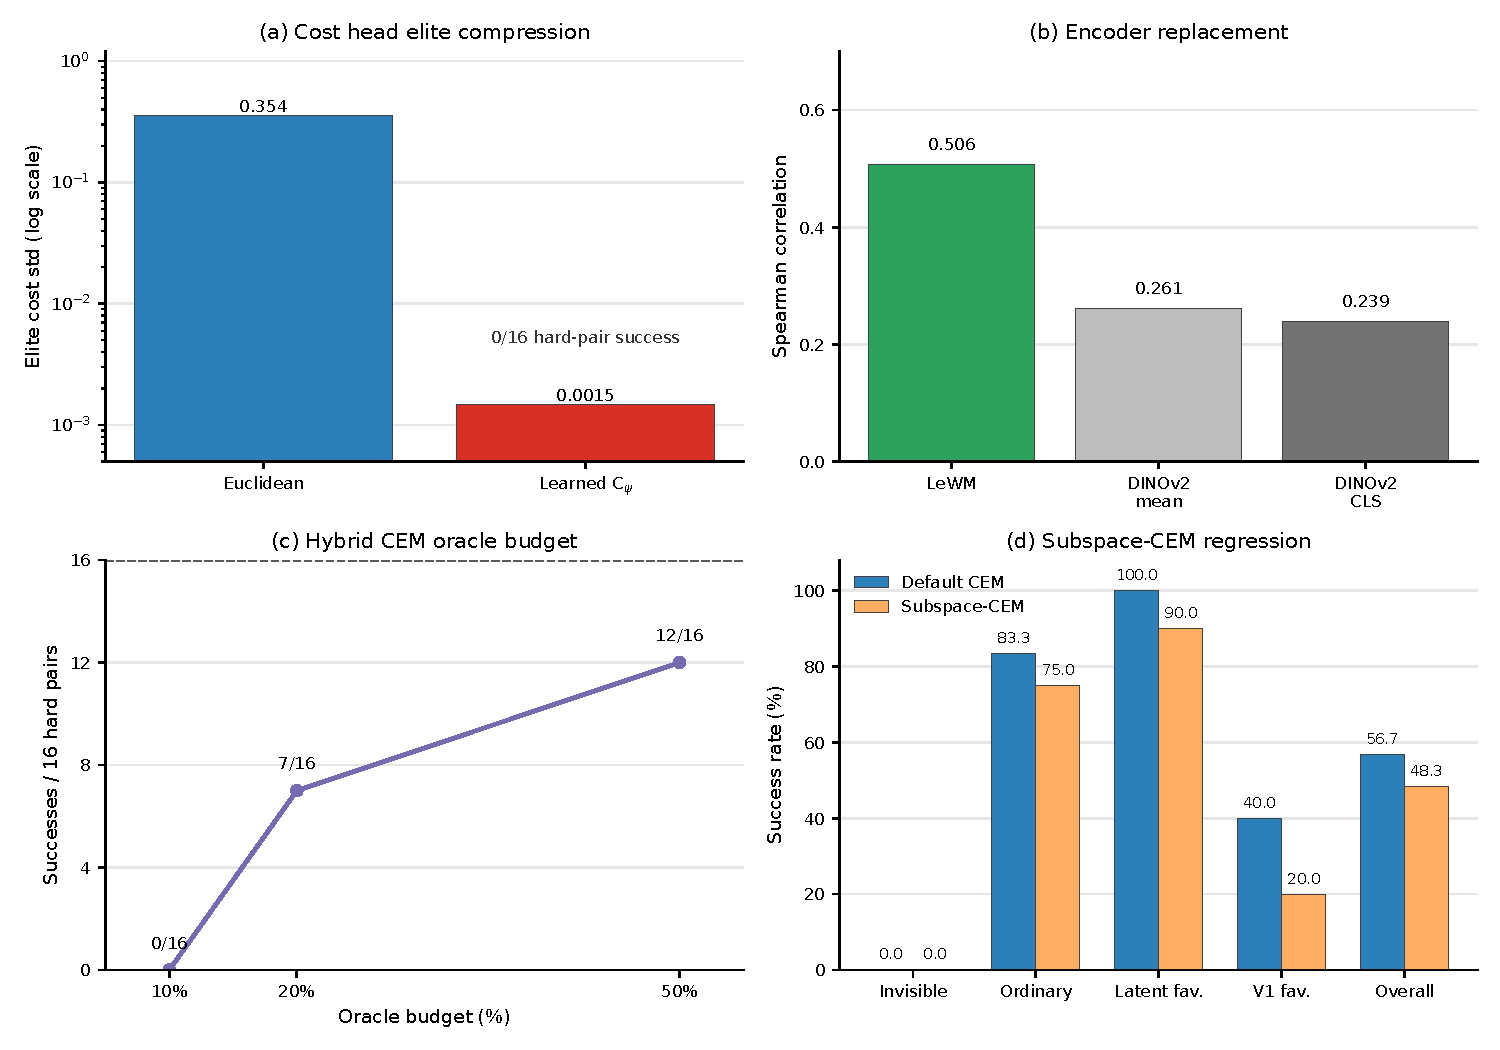
\includegraphics[width=\textwidth]{figures/figure4_negative_results.pdf}
\caption{Four failed repairs under locked criteria. \textbf{(a)}~Learned cost head $C_\psi$ compresses elite cost std by ${\sim}240\times$, removing local discrimination (0/16 hard-pair success). \textbf{(b)}~DINOv2 encoder replacement underperforms trained LeWM on endpoint ranking (0.261 vs.\ 0.506 Spearman). \textbf{(c)}~Hybrid CEM requires ${\geq}20\%$ oracle budget to recover any hard-pair successes. \textbf{(d)}~Subspace-CEM regresses across all subsets ($-8.3$\,pp overall).}
\label{fig:negative_results}
\end{figure}

Sections~4 and~5 establish that LeWM learns task-relevant endpoint geometry that can decouple from CEM-local planning behavior. We then tested four component-level repairs; each failed under its locked criterion.

\subsection{Learned cost heads}

The first repair replaced Euclidean latent distance with MLP cost heads $C_\psi(z,\zgoal)$ trained on V1 hinge labels over frozen LeWM latents. The large MLP improved held-out endpoint ranking (Spearman $0.479$ vs.\ $0.269$), but Figure~\ref{fig:negative_results} shows that elite costs collapsed and planning still failed.

\subsection{Encoder replacement}

The second repair swapped in DINOv2 ViT-B/14 (86.6M parameters, 768-dimensional features). Both variants underperformed trained LeWM on the same endpoint artifact (Figure~\ref{fig:negative_results}), so generic visual strength did not fix the cost landscape.

\subsection{Hybrid CEM}

The third repair re-ranked the top $K$ CEM candidates per iteration using the V1 simulator cost. Hybrid CEM needed a 20\% oracle budget before recovering any hard-pair successes (Figure~\ref{fig:negative_results}); $K=60$ adds $2.7\times$ wall-clock overhead, and $K=150$ requires millions of simulator steps.

\subsection{Subspace-CEM}

The fourth repair targeted the search-selection split found in Section~4: Subspace-CEM searched with an $m=64$ projected cost, then selected by full 192-dimensional LeWM cost. Under the locked Stage A criterion, this approach failed (Figure~\ref{fig:negative_results}), showing that projected-cost search can move the final pool into a region that full-dimensional re-ranking cannot repair.

\subsection{What the failures share}

Together, these locked failures point away from single-component repairs and toward the interaction between cost geometry and CEM dynamics---the object that endpoint-only metrics leave untested.
